\chapter{Definição do problema}

Diariamente novos dispositivos são inseridos no cotidiano da sociedade, essa variedade de "coisas" que fazem parte do cotidiano podem acabar se tornando um problema, principalmente para pessoas com pouca prática na conFiguração e utilização destes novos e modernos aparelhos. Neste ambiente desconexo, qualquer nova aquisição, como um novo ar condicionado ou uma fechadura eletrônica passam a ser mais um dispositivo com características novas e conFigurações diferentes que necessitam ser administrados por estes moradores.
As primeiras interfaces homem máquina (IHM) que utilizam o controle remoto, por rádio frequência, normalmente são as opções mais comuns e variadas nas residências atuais. A Figura \ref{controle} mostra algumas variações desta interface para controle das coisas de casa.

\begin{figure}[H]
\caption{\label{controle} Exemplos de IHM convencionais}
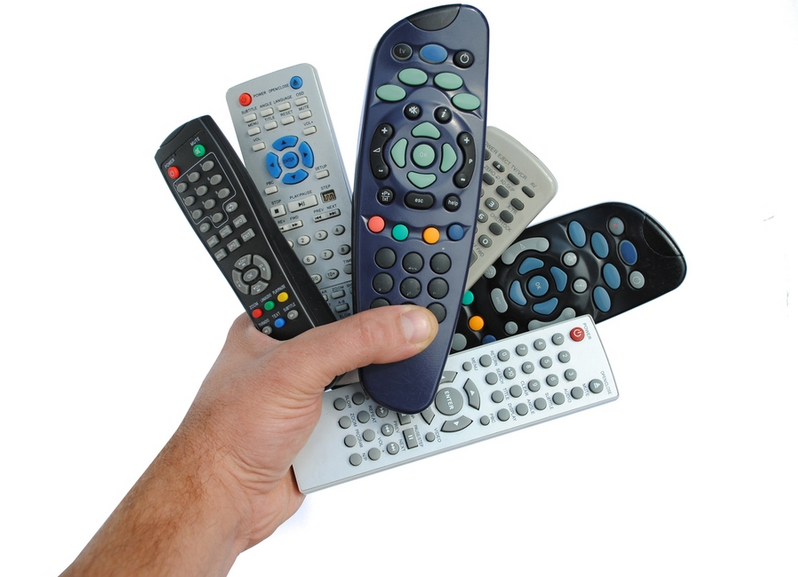
\includegraphics[scale=0.35]{img/controle-remoto.png}
\legend{Fonte: Website da digitaltrends}
\end{figure}

É comum que todos estes aparelhos funcionem de forma independente e desconectadas, cabendo aos usuários desvendar os segredos de cada IHM. O que deveria trazer facilidade e comodidade pode facilmente se tornar um forte motivo para aquela nova aquisição cair rapidamente em desuso ou simplesmente não ser utilizada da maneira correta. Outro cenário muito comum é a eleição de um "especialista" em novas tecnologias, as vezes um filho ou sobrinho descolado que domina as novidades recém chegadas. O fato é que esse acumulo de possibilidades gera insatisfação e porque não dizer frustração nos usuários que gostariam apenas de desfrutar das soluções e confortos que estes bens prometem trazer e nem sempre cumprem essa tarefa a contento.

Nos últimos anos, uma tendência tem se mostrado forte, a integração destes aparelhos, empresas grandes como Google\footnote{https://madeby.google.com/home/} , Amazon\footnote{https://www.amazon.com/dp/B00X4WHP5E} e Apple\footnote{https://www.apple.com/homepod} tem investido tempo e dinheiro para criar soluções que entregam uma experiência mais integrada ao cotidiano das pessoas. Este processo envolve a adaptação dos aparelhos existentes em conjunto com uma integração a novos sistemas e interfaces mais amigáveis. Todas as soluções citadas anteriormente utilizam o hábito dos moradores para fazer uma mapa e uma agenda de eventos, sugerindo com o passar do tempo certas ações que antes dependiam exclusivamente do controle humano, isso introduz o que convencionou chamar de Aprendizagem de Máquina associado a Sistemas de Recomendações. Estes sistemas prometem ser assistentes pessoais e conforme as demonstrações destes fabricantes, realmente vão mudar a maneira como nos relacionamos com as máquinas.

Neste processo, a captura de hábitos e o aprendizado que estas novas tecnologias prometem conseguir vão levar às próximas gerações a experimentar uma integração com as máquinas muito mais natural e porque não dizer orgânica. Fazer diferente o que de certa forma se acostuma pelo hábito é o que as soluções destas empresas propõem, interfaces de controle por voz, aprendizado de máquina e conexão com serviços externos são algumas das novidades que fazem parte do núcleo desta nova família de aplicativos e dispositivos.

Este mercado aposta em três itens para captar estes novos consumidores:
\begin{itemize}
    \item[a)] Conforto;
    \item[b)] Segurança;
    \item[c)] Integração.
\end{itemize}

Nem sempre a tecnologia costuma ficar disponível para a grande maioria de forma rápida, tornar projetos de eletrônica e informática uma realidade no Brasil muitas vezes é um desafio e isso por vezes nos deixa nos tempos das cavernas em relação a paises desenvolvidos, mesmo no mais otimista dos cenários ainda estamos longe de ter acesso as soluções de domótica existentes no exterior. As principais questões que dificultam o acesso a essas soluções são em primeiro lugar a falta de interesse comercial de trazer isso para nosso país, nossa infraestrutura embora tenha melhorado, ainda está longe do ideal. Os custos de serviço de \textit{telecom} associado as altas taxas de importação de eletrônicos inviabilizam a chegada destas facilidades as lojas do nosso país.
Estas dificuldades não vão fazer com que as pessoas deixem de querer isso e de alguma forma estas necessidades serão sanadas, dentro deste contexto que nasce o projeto de automação residencial chamado Ysto, este projeto se propõem a contemplar os itens acima citados de forma mais simples e a um uma fração do preço dos existentes na atualidade.

Fazer a aquisição de dados, transformá-los em informação útil e decidir o que fazer com esta informação disponibilizando uma interface simples e unificada será o escopo deste projeto, tudo isso a um custo mínimo. A Figura \ref{custos} mostra uma estimativa de preço para montagem de uma central de controle e um módulo auxiliar.

\begin{figure}[H]
\caption{\label{custos} Levantamento aproximado de custos}
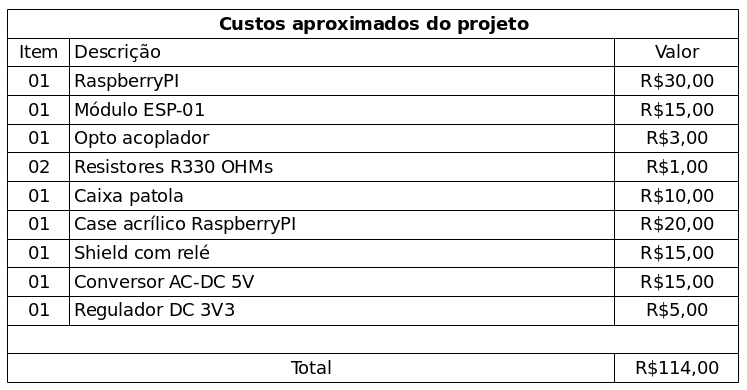
\includegraphics[scale=0.4]{img/custos.png}
\legend{Fonte: Autor do projeto}
\end{figure}

Estes valores foram coletados em sites como mercado livre e solda fria, são apenas estimativas e médias de preços, ou seja, podem variar. Uma alternativa muito interessante para aquisição dos componentes principais do sistema, a RaspberryPI e o ESP-01 são os sites chineses que disponibilizam estes componentes a preços muito mais atrativos. Apenas como efeito de ilustração, o site Aliexpress vende conjuntos de cinco ESP-01 a R\$32,00 é possível optar por um módulo pronto como o da Figura \ref{modulo-ali}.

\begin{figure}[H]
\caption{\label{modulo-ali} Alternativa pronta para o MA}
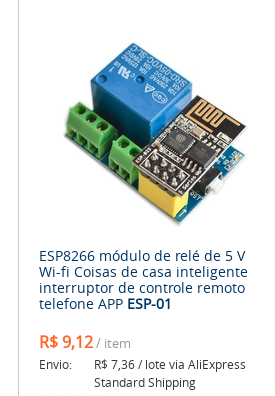
\includegraphics[scale=0.4]{img/modulo-ali.png}
\legend{Fonte: Website da Aliexpress}
\end{figure}

Este módulo reduziria nosso custo para aproximadamente R\$60.00 e teríamos algo muito prático e de fácil utilização.


